\documentclass[aspectratio=169,10pt]{beamer}
\usepackage[T1]{fontenc}
\usepackage{lmodern}
\usetheme[progressbar=frametitle]{metropolis}
\definecolor{accent}{HTML}{548E9B}
\setbeamercolor{frametitle}{bg=accent, fg=white}
\setbeamercolor{progress bar}{fg=accent}
\setbeamercolor{title separator}{fg=accent}
\setbeamercolor{alerted text}{fg=accent}

% figure helper: width-bound to the text width, height capped by the optional factor
\newcommand{\slidefig}[2][0.5]{\par\vspace{0.5ex}{\centering
  \includegraphics[width=\textwidth,height=#1\textheight,keepaspectratio]{figures/#2}\par}\vspace{0.5ex}}

\title{Deep models reveal better strategies for superposition}
\author{Bartosz Rzepkowski\\[2ex]
  {\small Research Manager: Philipp Alexander Kreer\\
  Mentors: Thomas Dooms and Logan Riggs}}
\date{}

\begin{document}

\frame{\titlepage}

\begin{frame}{Introduction}
\begin{itemize}
  \item This work is heavily inspired by the \href{https://transformer-circuits.pub/2022/toy_model/index.html}{\emph{Toy Models of Superposition}} work.
  \item In the original paper the authors studied toy autoencoders consisting of two layers with a ReLU activation, and a bottleneck after the first layer.
\end{itemize}
\end{frame}

\begin{frame}{Introduction}
\begin{itemize}
  \item The input consisted of numbers $x_i$ (\textbf{features}), which could activate with a probability $p$, or remain inactive. When they became active, they took values in the $[0,1]$ range.
  \item Each feature can be given an additional importance weight.
  \item The error was measured using MSE.
\end{itemize}
\end{frame}

\begin{frame}{Introduction}
\begin{itemize}
  \item At the bottleneck, each feature $x_i$ is represented by its \textbf{embedding} vector $f_i$.
  \item The main result of \emph{Toy Models of Superposition} is that for sparse enough features (small value of $p$) the model stores more features than the bottleneck has dimensions (superposition).
\end{itemize}
\slidefig[0.56]{gallery_bilinear1.pdf}
\end{frame}

\begin{frame}{Introduction}
\begin{itemize}
  \item \emph{Toy Models of Superposition} observes deformed, non-uniform geometries only when the features themselves are non-uniform --- differing in importance, sparsity, or being correlated.
  \item \textbf{For identical features, however, it finds regular geometric structures, such as antipodal pairs, triangles and pentagons. Its authors remark that this structure ``seems `too elegant to be true'\,'' and that ``there's a good chance it's at least partly idiosyncratic to the toy model we're investigating''.}
\end{itemize}
\end{frame}

\begin{frame}{Introduction}
\begin{itemize}
  \item This work confirms this suspicion. It turns out that non-symmetric solutions give better performance, but the shallow models are just not expressive enough to ``discover'' them.
  \item In this work we study deeper models, which, thanks to their increased expressivity, discover better ``strategies'' resulting in a smaller MSE.
  \item We also introduce the theoretically best possible solution to this task (like a model with infinite expressivity), and use it as a benchmark to compare against when analyzing our models.
\end{itemize}
\end{frame}

\begin{frame}{Setup}
\begin{itemize}
  \item We will be working with models consisting of a linear encoder followed by multiple MLPs with a bilinear activation:
\end{itemize}
\slidefig[0.69]{setup_diagram.png}
\end{frame}

\begin{frame}{Setup}
\begin{itemize}
  \item For our analysis we divide the model into two parts:
  \begin{itemize}
    \item \textbf{Encoder}: consisting of the first linear layer.
    \item \textbf{Decoder}: consisting of all the following MLPs.
  \end{itemize}
  \item Each model will be given 4 features, all with the same $p = 0.2$.
  \item The encoder introduces the bottleneck, which forces the feature embeddings to live in a 2D space.
  \item We will analyze the geometries of feature embeddings precisely at this bottleneck.
\end{itemize}
\end{frame}

\begin{frame}{Let's play a game}
\begin{itemize}
  \item Imagine that you and your friend are playing a game.
  \item You are the encoder, and your goal is to arrange the feature embeddings in such a way that will make your friend's (the decoder's) life easier.
  \item That is, you should come up with the best possible arrangement of 4 feature embeddings to maximize the chances that your friend will guess correctly what the true input was before going through the bottleneck.
\end{itemize}
\end{frame}

\begin{frame}{Trivial strategy}
\begin{itemize}
  \item The trivial strategy is to pair the features, and arrange them in the following way:
\end{itemize}
\slidefig[0.6]{naive_cross.png}
\end{frame}

\begin{frame}{Trivial strategy}
\begin{itemize}
  \item Let's focus for now on the horizontal line segment spanned by the $f_1$ and $f_3$ feature embeddings. Let's denote it as $s$.
  \item This arrangement has one flaw. When two features in the same pair are co-active, the decoder cannot perfectly distinguish this case from a scenario in which only one of them was active:
\end{itemize}
\slidefig[0.51]{naive_cases.png}
\end{frame}

\begin{frame}{Trivial strategy}
\begin{itemize}
  \item In order to make the best possible prediction, he would have to \textbf{average} over these two clashing scenarios.
  \item You might ask: ``Why should the decoder use the average? Can't he use the median or the maximum instead?''
  \item This comes from the fact that we are using MSE to measure the performance of the whole system.
\end{itemize}
\end{frame}

\begin{frame}{Interlude - MSE}
\begin{itemize}
  \item Let's imagine you are given a bunch of points on a vertical line. (The unusual choice of vertical direction will become clear in a few slides.)
  \item You can output \textbf{just a single point}.
  \item The value you output will be compared with all the points that you were given.
  \item The sum of squared distances to each of these points is your final ``score'', and you should make it as small as possible.
  \item What should you do?
\end{itemize}
\end{frame}

\begin{frame}{Interlude - MSE}
\begin{itemize}
  \item It turns out that the best you can do in this situation is to just output the average of the points that were presented to you:
\end{itemize}
\slidefig[0.58]{mse_average.pdf}
\begin{itemize}
  \item This shows that \textbf{the choice of the loss function dictates the behavior of the decoder}.
\end{itemize}
\end{frame}

\begin{frame}{Trivial strategy - decoder's action}
\begin{itemize}
  \item We've shown that the decoder should use the average to achieve his goal. But how should he use it given the reading on the horizontal line segment $s$?
  \item Let's first take a look at what the decoder is seeing, when given a bunch of samples and trying to predict the true value of the feature $x_1$:
\end{itemize}
\slidefig[0.56]{samples_x1_sym.pdf}
\end{frame}

\begin{frame}{Trivial strategy - decoder's action}
\begin{itemize}
  \item We can clearly see that cases with both features active (green) fall on the same values of $s$ as other cases.
  \item The decoder can account for that as follows:
  \begin{itemize}
    \item divide $s$ into very tiny bins,
    \item for each such bin collect all the samples that fall into it,
    \item return the prediction of the first feature (denoted as $\hat{x}_1$) as the average of these points.
  \end{itemize}
\end{itemize}
\end{frame}

\begin{frame}{Trivial strategy - decoder's action}
\begin{itemize}
  \item Below we show one such bin. The samples inside it are spread along the vertical direction, which justifies our previous choice in the ``MSE interlude'':
\end{itemize}
\slidefig[0.68]{samples_x1_bin.pdf}
\end{frame}

\begin{frame}{Trivial strategy - decoder's action}
\begin{itemize}
  \item With very fine bins, the decoder's predictions (the blue line) look as follows:
\end{itemize}
\slidefig[0.74]{binned_x1_sym.pdf}
\end{frame}

\begin{frame}{Trivial strategy - decoder's action}
\begin{columns}[c]
\begin{column}{0.52\textwidth}
\begin{itemize}
  \item The black curve is the closed-form solution: the best possible prediction the decoder can make.
  \item Deriving it is quite difficult and requires knowing the true data-generating process --- something we usually lack, having access only to data samples.
  \item Still, with infinitely many samples and infinitely narrow bins, the binned predictions would converge to the closed form.
  \item From now on, we will switch between the closed-form solution and the binned average, whichever is more convenient.
\end{itemize}
\end{column}
\begin{column}{0.48\textwidth}
\centering
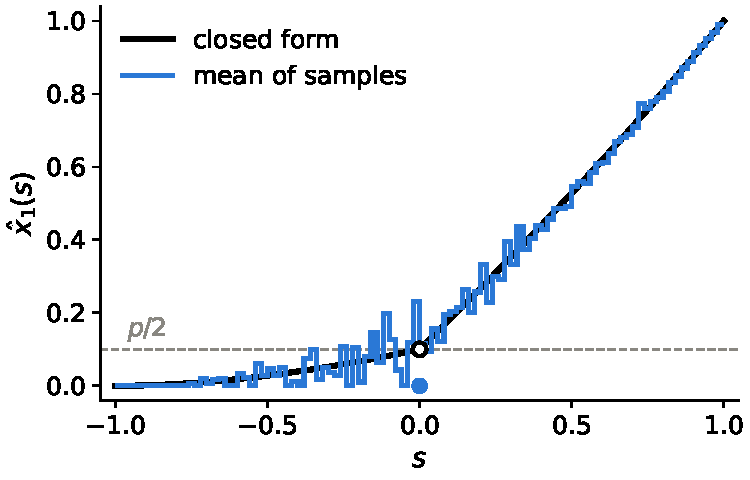
\includegraphics[width=\textwidth]{figures/binned_x1_sym.pdf}
\end{column}
\end{columns}
\end{frame}

\begin{frame}{Trivial strategy - decoder's action}
\begin{itemize}
  \item We should remember that readings on the same line segment $s$ are used to predict both $\hat{x}_1$ and $\hat{x}_3$. Let's plot them together.
\end{itemize}
\slidefig[0.6]{posterior_pair_sym.pdf}
\end{frame}

\begin{frame}{Better strategies - making feature embeddings asymmetrical}
\begin{itemize}
  \item The above decoders were the best possible ones for the \textbf{symmetrical feature embeddings}.
  \item However, we can make these features asymmetrical:
\end{itemize}
\slidefig{levers.png}
\end{frame}

\begin{frame}{Better strategies - making feature embeddings asymmetrical}
\begin{itemize}
  \item We can derive the best theoretical decoders for this new geometry, and obtain the following result:
\end{itemize}
\slidefig[0.59]{asym_compare_wide.pdf}
\begin{itemize}
  \item We can see that \textbf{the asymmetrical approach gives a smaller overall MSE!}
\end{itemize}
\end{frame}

\begin{frame}{Better strategies - opening the pair}
\begin{itemize}
  \item Another way to improve the decoder's chances is to ``open'' the feature embedding pair:
\end{itemize}
\slidefig[0.3]{opening.png}
\begin{itemize}
  \item With this setup:
  \begin{itemize}
    \item in a situation with just a single feature being active, we still get a reading on one of the feature embeddings,
    \item when two features are co-active we get a reading inside the parallelogram spanned by the feature embeddings, which is distinguishable from the case with just a single feature being active.
  \end{itemize}
\end{itemize}
\end{frame}

\begin{frame}{Better strategies - opening the pair}
\begin{itemize}
  \item This approach is not perfect, however. We need to remember that we have to store four different embeddings in a 2D plane.
\end{itemize}
\slidefig[0.68]{opened_geometry_plain.pdf}
\end{frame}

\begin{frame}{Better strategies - opening the pair}
\begin{columns}[c]
\begin{column}{0.52\textwidth}
\begin{itemize}
  \item Thus, tilting the $f_3$ feature embedding makes it overlap with the $f_2$ one --- we will call this effect the \textbf{interference} between features.
  \item Still, this strategy is better than not tilting at all: to get a reading on the overlapping line segment, $x_1$ and $x_3$ would have to be co-active \textbf{and} produce a reading landing exactly on the $f_2$ embedding, which is extremely rare.
\end{itemize}
\end{column}
\begin{column}{0.46\textwidth}
\centering
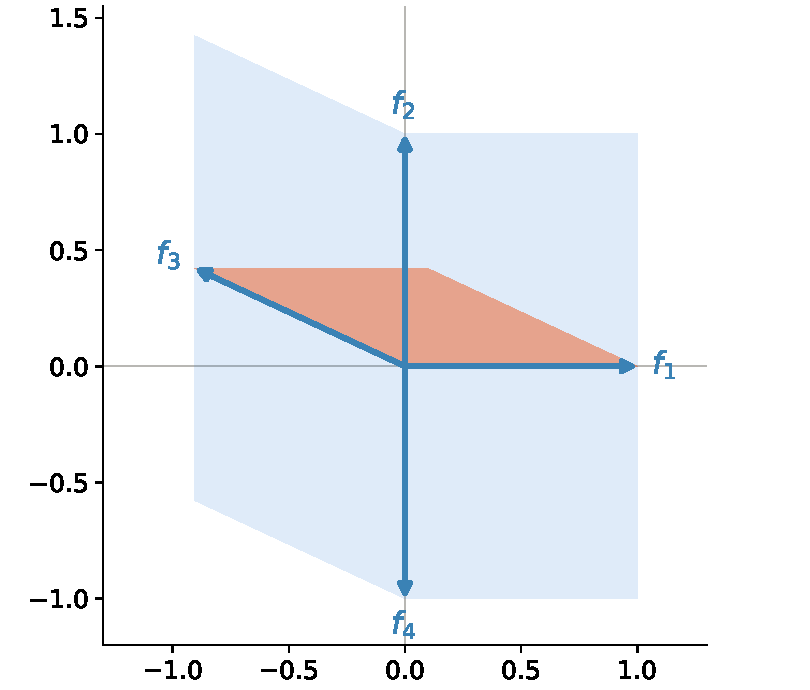
\includegraphics[width=\textwidth]{figures/opened_geometry_plain.pdf}
\end{column}
\end{columns}
\end{frame}

\begin{frame}{Best possible strategy}
To summarize, the \textbf{best possible strategy should balance three mechanisms}:
\begin{itemize}
  \item It can make the embeddings of a pair \textbf{asymmetrical}, which lowers the overall MSE,
  \item It can \textbf{tilt} the pairs open, so that co-activation can be told apart from a single active feature,
  \item But at the same time it needs to account for the \textbf{interference} with the other pair's features.
\end{itemize}
\end{frame}

\begin{frame}{Best possible strategy}
\begin{itemize}
  \item We can find the theoretically best possible arrangement of embeddings by changing their length and tilt, and scoring the final result using the binned decoder (with bins being in this case small 2D squares instead of extremely short line segments).
  \item This kind of search results in the following arrangement:
\end{itemize}
\slidefig[0.57]{optimal_geometry.pdf}
\end{frame}

\begin{frame}{Best possible strategy}
\begin{columns}[c]
\begin{column}{0.54\textwidth}
\begin{itemize}
  \item We can notice that the paired features are clearly asymmetrical and tilted.
  \item But the $f_1$ and $f_2$ embeddings came out much shorter than simply using the asymmetry to reduce the MSE within each pair would suggest.
  \item It turns out that they are shortened in order to reduce the aforementioned interference.
\end{itemize}
\end{column}
\begin{column}{0.44\textwidth}
\centering
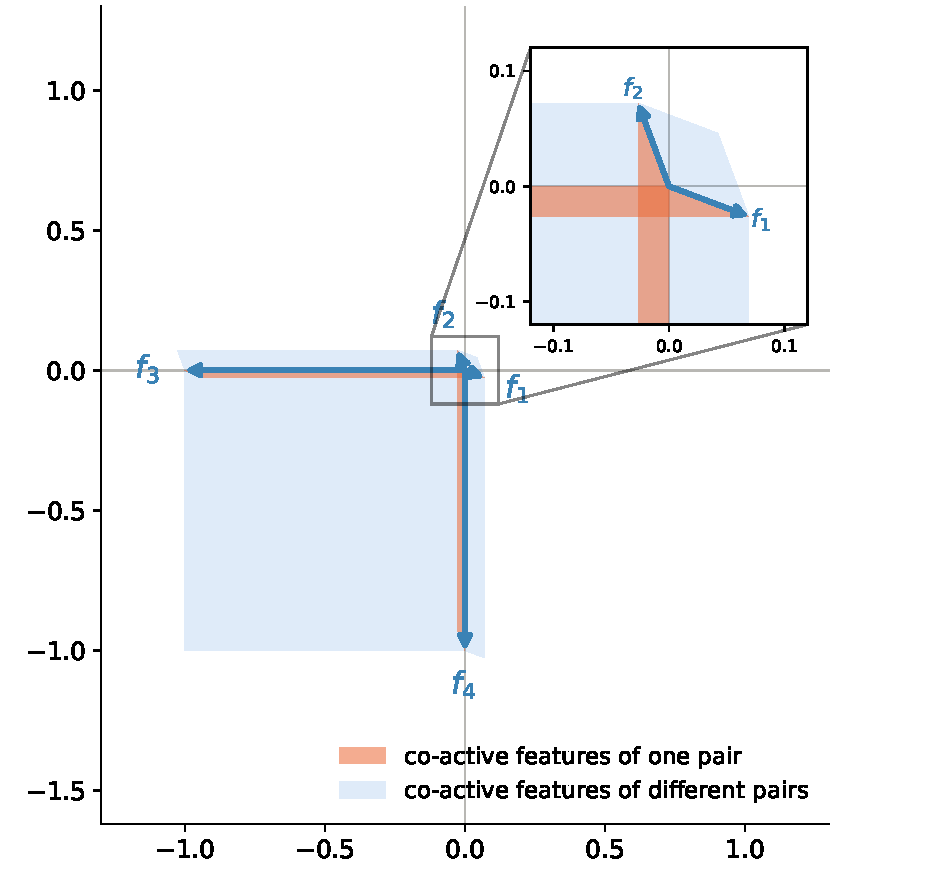
\includegraphics[width=\textwidth]{figures/optimal_geometry.pdf}
\end{column}
\end{columns}
\end{frame}

\begin{frame}{The actual arrangements discovered by the models}
\begin{itemize}
  \item So far we have been exploring the geometries that could be utilized by the best possible decoder.
  \item But what do the geometries discovered by the actual models look like?
\end{itemize}

\end{frame}

\begin{frame}{The actual arrangements discovered by the models}
\begin{itemize}
  \item We can compare the representative results from a model with only a single bilinear MLP (shallow) vs a model with four such layers (deep):
\end{itemize}
\slidefig{gallery.pdf}
\begin{itemize}
  \item Clearly, only the deeper model utilizes the strategies mentioned previously. Why is that?
\end{itemize}
\end{frame}

\begin{frame}{Why do only deep models utilize asymmetry?}
\begin{itemize}
  \item The depth of a model corresponds to its expressivity. A model with a single bilinear MLP can be understood as a 2nd-degree polynomial, while the model with four MLPs is a 16th-degree polynomial.
  \item With this in mind and having the best theoretical decoder as a benchmark, we can look for the best-in-class approximation of the unconstrained solution.
\end{itemize}
\end{frame}

\begin{frame}{Why do only deep models utilize asymmetry?}
\begin{itemize}
  \item Below we show the theoretical decoder in gray, together with its approximations as the colored curves.
  \item For a 2nd-degree polynomial (shallow model) we can clearly see that it approximates the symmetrical case better than the asymmetrical one:
\end{itemize}
\slidefig[0.4]{class_quadratic.pdf}
\begin{itemize}
  \item Because of that it will default to the symmetrical case.
\end{itemize}
\end{frame}

\begin{frame}{Why do only deep models utilize asymmetry?}
\begin{itemize}
  \item The 16th-degree polynomial (deep model) has no problem approximating both the symmetrical and asymmetrical cases, so it chooses the one which gives a smaller overall MSE:
\end{itemize}
\slidefig[0.55]{class_deg16.pdf}
\end{frame}

\begin{frame}{Why do only deep models utilize asymmetry?}
\begin{itemize}
  \item We also studied the model investigated in the \emph{Toy Models of Superposition} paper.
  \item Similarly to the shallow bilinear model, it cannot properly approximate the asymmetrical solution, so it will default to the symmetrical one:
\end{itemize}
\slidefig[0.5]{class_relu_tied.pdf}
\end{frame}

\begin{frame}{Why do only deep models utilize tilt?}
\begin{itemize}
  \item To understand why only deeper models utilize the tilting of the pair, we can run a similar experiment.
  \item This time we will fix the geometry to the previously shown case, with just one embedding being slightly tilted. We will focus on the line segment cutting the plane as shown below:
\end{itemize}
\slidefig[0.56]{opened_geometry.pdf}
\end{frame}

\begin{frame}{Why do only deep models utilize tilt?}
\begin{itemize}
  \item For this arrangement we can fit the binned decoder as well as constrained functions corresponding to the models with bilinear and ReLU activations.
  \item Below we can see the results of the fitting procedure:
\end{itemize}
\slidefig[0.62]{opened_decoded.pdf}
\end{frame}

\begin{frame}{Why do only deep models utilize tilt?}
\begin{columns}[c]
\begin{column}{0.46\textwidth}
\begin{itemize}
  \item It turns out that, again, the expressivity of the model explains why it can or cannot use the tilting.
  \item The binned decoder can very efficiently detect this opening of a pair. The shallow models are too simple to detect such a narrow opening. Only models with 3 and 4 bilinear MLPs are expressive enough to detect the opening.
\end{itemize}
\end{column}
\begin{column}{0.52\textwidth}
\centering
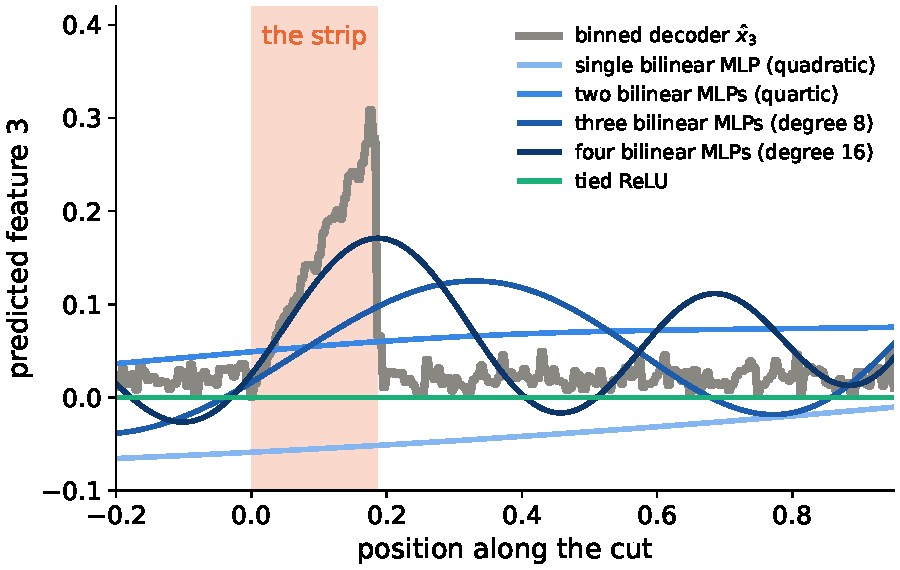
\includegraphics[width=\textwidth]{figures/opened_decoded.pdf}
\end{column}
\end{columns}
\end{frame}

\begin{frame}{Summary}
\begin{itemize}
  \item We've shown that the symmetrical geometries formed by the feature embeddings, discovered in \emph{Toy Models of Superposition} in experiments with features of equal importance and sparsity, and with no correlation, are an artifact of the chosen model architecture rather than a general phenomenon.
  \item We've presented several asymmetrical strategies, which the models can use to reduce the overall MSE.
  \item Only deep models can utilize these strategies, thanks to their greater expressivity compared to their shallow counterparts.
\end{itemize}
\end{frame}

\end{document}
